
\chapter{Radio Scattering}

\section{Scattering Basics, and the $\alpha=-4$ Scattering Index}

Scattering causes radiation to follow different paths
through an inhomogeneous plasma. Since these paths have
different lengths, radiation emitted simultaneously can
arrive at different times, broadening the observed pulse.

We will derive the frequency dependence of this
broadening, assuming a thin scattering screen, small
scattering angles, and a characteristic transverse plasma
structure that does not change with observing frequency.

\subsubsection{How a Plasma Bends Light}

Recall that the refractive index of a cold plasma is

\begin{equation}
n=\sqrt{1-\frac{\omega_p^2}{\omega^2}}.
\end{equation}

Using

\begin{equation}
\omega_p^2=\frac{n_e e^2}{\epsilon_0 m_e},
\end{equation}

and assuming $\omega\gg\omega_p$, we can expand
$\sqrt{1-u}\simeq 1-u/2$ to obtain

\begin{equation}
n \simeq 1 -
\frac{n_e e^2}{2\epsilon_0 m_e\omega^2}.
\end{equation}

Therefore,

\begin{equation}
\boxed{n-1\propto -n_e\nu^{-2}.}
\end{equation}

The refractive index depends on both the electron
density and the observing frequency.

If the electron density changes across the wavefront,
different parts of the wave travel at different phase
velocities. This causes the wavefront to rotate,
changing the direction of propagation.

We can understand this using Snell's law:

\begin{equation}
n_1\sin\phi_1=n_2\sin\phi_2,
\end{equation}

where $\phi$ is measured relative to the normal of
the boundary between the two media.

\begin{center}
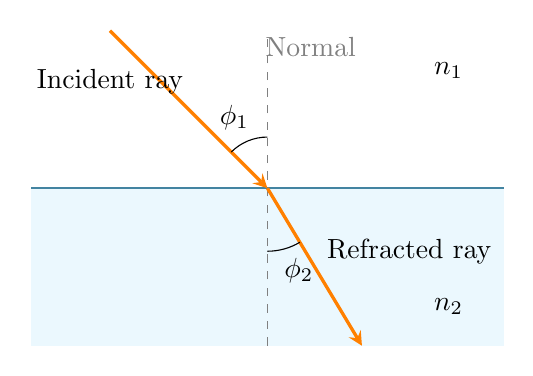
\begin{tikzpicture}[scale=1.0,>=stealth]
    % Two media
    \fill[cyan!8] (-3,-2) rectangle (3,0);
    \draw[cyan!60!black,thick] (-3,0)--(3,0);

    % Boundary normal
    \draw[dashed,gray] (0,-2)--(0,2);

    % Incident and refracted rays
    \draw[very thick,orange,->] (-2,2)--(0,0);
    \draw[very thick,orange,->] (0,0)--(1.2,-2);

    % Angles measured from normal
    \draw (0,0.65)
        arc[start angle=90,end angle=135,radius=0.65];
    \node at (-0.42,0.9) {$\phi_1$};

    \draw (0,-0.8)
        arc[start angle=270,end angle=301,radius=0.8];
    \node at (0.4,-1.05) {$\phi_2$};

    % Labels
    \node at (2.3,1.5) {$n_1$};
    \node at (2.3,-1.5) {$n_2$};
    \node[gray] at (0.55,1.8) {Normal};
    \node at (-2.0,1.35) {Incident ray};
    \node at (1.8,-0.8) {Refracted ray};
\end{tikzpicture}
\end{center}

Consider two adjacent regions with refractive indices
$n$ and $n+dn$. A ray crossing their boundary obeys

\begin{equation}
n\sin\phi=(n+dn)\sin(\phi+d\phi).
\end{equation}

Using the angle-addition formula,

\begin{equation}
\sin(\phi+d\phi)
=
\sin\phi\cos(d\phi)
+
\cos\phi\sin(d\phi).
\end{equation}

For an infinitesimal angle $d\phi$,

\begin{equation}
\cos(d\phi)\simeq 1,
\qquad
\sin(d\phi)\simeq d\phi.
\end{equation}

Therefore,

\begin{equation}
\sin(\phi+d\phi)
\simeq
\sin\phi+\cos\phi\,d\phi.
\end{equation}

Substituting into Snell's law,

\begin{equation}
n\sin\phi
\simeq
(n+dn)(\sin\phi+\cos\phi\,d\phi).
\end{equation}

Expanding and neglecting the second-order
term $dn\,d\phi$,

\begin{equation}
n\sin\phi
\simeq
n\sin\phi
+dn\sin\phi
+n\cos\phi\,d\phi.
\end{equation}

Subtracting $n\sin\phi$ from both sides,

\begin{equation}
0=dn\sin\phi+n\cos\phi\,d\phi.
\end{equation}

Rearranging,

\begin{equation}
n\cos\phi\,d\phi=-dn\sin\phi,
\end{equation}

so

\begin{equation}
\boxed{
d\phi=-\frac{\tan\phi}{n}\,dn.
}
\end{equation}

This equation describes how the ray's angle relative
to the boundary normal changes when it crosses a
small change in refractive index.

However, we ultimately want to know how the ray's
direction changes as it propagates through the plasma.

To do this, we must introduce a coordinate system.

\paragraph{Introducing the $x$ and $z$ Coordinates}

We choose our coordinates such that

\begin{itemize}
    \item $z$ is the direction in which the ray
    approximately propagates.
    \item $x$ is the transverse direction,
    perpendicular to $z$.
    \item $\theta$ is the angle the ray makes
    with the $z$-axis.
    \item $\phi$ is the angle the ray makes
    with the $x$-axis, which is normal to
    the refractive-index boundary.
\end{itemize}

For the moment, suppose the refractive index
varies only in the transverse direction,

\begin{equation}
n=n(x).
\end{equation}

The surfaces of constant refractive index are
therefore parallel to the $z$-axis.

\begin{center}
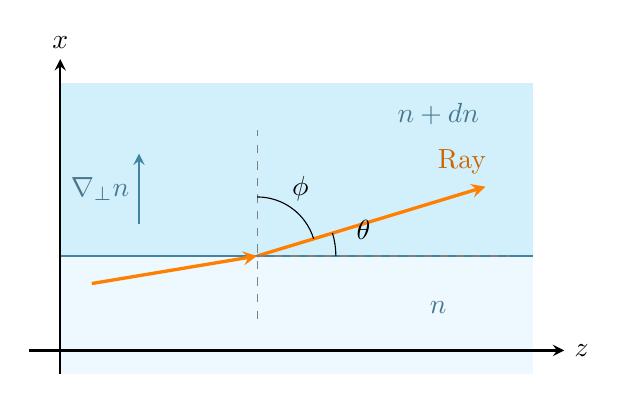
\begin{tikzpicture}[scale=1.0,>=stealth]

    % Refractive index regions
    \fill[cyan!7] (0,-1.5) rectangle (6,0);
    \fill[cyan!18] (0,0) rectangle (6,2.2);

    % Boundary
    \draw[cyan!60!black,thick]
        (0,0)--(6,0);

    % Coordinate axes
    \draw[->,thick]
        (0,-1.5)--(0,2.5)
        node[above] {$x$};

    \draw[->,thick]
        (-0.4,-1.2)--(6.4,-1.2)
        node[right] {$z$};

    % Incoming ray
    \draw[very thick,orange,->]
        (0.4,-0.35)--(2.5,0);

    % Refracted ray
    \draw[very thick,orange,->]
        (2.5,0)--(5.4,0.88);

    % Normal to boundary
    \draw[dashed,gray]
        (2.5,-0.8)--(2.5,1.6);

    % Reference propagation direction
    \draw[dashed,gray]
        (2.5,0)--(5.7,0);

    % Theta relative to z
    \draw
        (3.5,0)
        arc[start angle=0,end angle=17,radius=1];

    \node at (3.85,0.33) {$\theta$};

    % Phi relative to x
    \draw
        (2.5,0.75)
        arc[start angle=90,end angle=17,radius=0.75];

    \node at (3.05,0.85) {$\phi$};

    % Refractive index labels
    \node[cyan!50!black] at (4.8,1.8) {$n+dn$};
    \node[cyan!50!black] at (4.8,-0.65) {$n$};

    % Transverse gradient
    \draw[->,cyan!60!black,thick]
        (1.0,0.4)--(1.0,1.3);

    \node[cyan!50!black,left]
        at (1.0,0.85)
        {$\nabla_\perp n$};

    \node[orange!80!black]
        at (5.1,1.2) {Ray};

\end{tikzpicture}
\end{center}

The important distinction is that $\phi$ and
$\theta$ describe the same ray, but are measured
relative to different axes.

Since the $x$ and $z$ axes are perpendicular,

\begin{equation}
\boxed{
\theta=\frac{\pi}{2}-\phi.
}
\end{equation}

Differentiating,

\begin{equation}
\boxed{d\theta=-d\phi.}
\end{equation}

Thus, an increase in $\phi$ corresponds to a
decrease in $\theta$, and vice versa.

We can now rewrite our Snell's-law result
in terms of $\theta$.

Starting with

\begin{equation}
d\phi=-\frac{\tan\phi}{n}\,dn,
\end{equation}

and using $d\theta=-d\phi$, we obtain

\begin{equation}
d\theta=\frac{\tan\phi}{n}\,dn.
\end{equation}

\paragraph{Relating the Angles to Distance}

From the geometry, the tangent of $\phi$ is

\begin{equation}
\boxed{
\tan\phi=\frac{dz}{dx}.
}
\end{equation}

This follows because $\phi$ is measured from
the $x$-axis, so $dz$ is the opposite side
and $dx$ is the adjacent side.

Equivalently,

\begin{equation}
\tan\theta=\frac{dx}{dz}.
\end{equation}

For a ray travelling nearly parallel to $z$,
$\theta\ll 1$, and therefore

\begin{equation}
\theta\simeq\frac{dx}{dz}.
\end{equation}

Next, because the refractive index depends on
the transverse coordinate $x$, a small change
$dx$ produces a change in refractive index

\begin{equation}
\boxed{
dn=\frac{\partial n}{\partial x}\,dx.
}
\end{equation}

This is simply the first-order change in
$n(x)$ as we move a distance $dx$ in the
transverse direction.

We now substitute both expressions into

\begin{equation}
d\theta=\frac{\tan\phi}{n}\,dn.
\end{equation}

This gives

\begin{equation}
d\theta=
\frac{1}{n}
\underbrace{\frac{dz}{dx}}_{\tan\phi}
\underbrace{
\frac{\partial n}{\partial x}\,dx
}_{dn}.
\end{equation}

The factors of $dx$ cancel, leaving

\begin{equation}
\boxed{
d\theta=
\frac{1}{n}
\frac{\partial n}{\partial x}\,dz.
}
\end{equation}

Dividing by $dz$,

\begin{equation}
\boxed{
\frac{d\theta}{dz}
=
\frac{1}{n}\frac{\partial n}{\partial x}.
}
\end{equation}

This equation has a simple physical interpretation:

\begin{equation}
\underbrace{
\frac{d\theta}{dz}
}_{\substack{\text{Change in ray direction}\\
\text{per unit distance}}}
=
\underbrace{
\frac{1}{n}\frac{\partial n}{\partial x}
}_{\substack{\text{Transverse gradient}\\
\text{in refractive index}}}.
\end{equation}

A ray bends toward the direction of increasing
refractive index.

If the refractive index is uniform in the
transverse direction,

\begin{equation}
\frac{\partial n}{\partial x}=0,
\end{equation}

then

\begin{equation}
\frac{d\theta}{dz}=0.
\end{equation}

The ray therefore travels in a straight line.

Conversely, a transverse gradient in refractive
index causes the ray's direction to change
as it propagates along $z$.

For a tenuous plasma, $n\simeq 1$, giving

\begin{equation}
\boxed{
\frac{d\theta}{dz}
\simeq
\frac{\partial n}{\partial x}.
}
\end{equation}

This is the small-angle ray-bending equation.

Although we introduced it using the special
case $n=n(x)$, the same leading-order equation
holds for a general weakly refracting plasma
with $n=n(x,z)$. In that case, it follows
from the geometrical-optics ray equation,
evaluated along the nearly straight ray path.

\paragraph{Integrating Through a Plasma Screen}

Consider a ray passing through a plasma screen
with a transverse refractive-index gradient.

\begin{center}
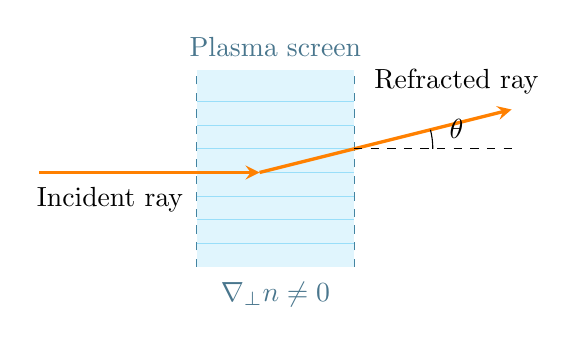
\begin{tikzpicture}[scale=1.0,>=stealth]

    % Plasma screen
    \fill[cyan!12]
        (2,-1.2) rectangle (4,1.3);

    \draw[cyan!60!black,dashed]
        (2,-1.2)--(2,1.3);

    \draw[cyan!60!black,dashed]
        (4,-1.2)--(4,1.3);

    % Density layers
    \foreach \y in {-0.9,-0.6,...,0.9} {
        \draw[cyan!40]
            (2,\y)--(4,\y);
    }

    \node[cyan!50!black]
        at (3,1.6) {Plasma screen};

    \node[cyan!50!black]
        at (3,-1.55)
        {$\nabla_\perp n\neq 0$};

    % Incoming and outgoing ray
    \draw[very thick,orange,->]
        (0,0)--(2.8,0);

    \draw[very thick,orange]
        (2.8,0)--(4,0.3);

    \draw[very thick,orange,->]
        (4,0.3)--(6,0.8);

    % Reference direction
    \draw[dashed]
        (4,0.3)--(6,0.3);

    % Angle
    \draw
        (5,0.3)
        arc[start angle=0,end angle=14,radius=1];

    \node at (5.3,0.55) {$\theta$};

    \node at (0.9,-0.35) {Incident ray};
    \node at (5.3,1.15) {Refracted ray};

\end{tikzpicture}
\end{center}

The ray's direction changes continuously
as it travels through the screen.

To find the total angular deflection,
we integrate the ray-bending equation
over the thickness of the plasma.

For an initially undeflected ray,

\begin{equation}
\theta_{\rm def}
\simeq
\int_{\rm screen}
\frac{\partial n}{\partial x}\,dz.
\end{equation}

Here $\theta_{\rm def}$ is the net change in
the ray's direction as it crosses the screen.

Substituting the plasma refractive index,

\begin{equation}
n\simeq
1-\frac{n_e e^2}{2\epsilon_0m_e\omega^2},
\end{equation}

we first calculate the transverse derivative:

\begin{equation}
\frac{\partial n}{\partial x}
=
-\frac{e^2}{2\epsilon_0m_e\omega^2}
\frac{\partial n_e}{\partial x}.
\end{equation}

Therefore,

\begin{equation}
\theta_{\rm def}
\simeq
-\frac{e^2}{2\epsilon_0m_e\omega^2}
\int_{\rm screen}
\frac{\partial n_e}{\partial x}\,dz.
\end{equation}

Define the electron column density through
the screen as

\begin{equation}
N_e(x)=
\int_{\rm screen}n_e(x,z)\,dz.
\end{equation}

Assuming the screen boundaries are fixed,
we can interchange the derivative and integral:

\begin{equation}
\frac{\partial N_e}{\partial x}
=
\int_{\rm screen}
\frac{\partial n_e}{\partial x}\,dz.
\end{equation}

Thus,

\begin{equation}
\boxed{
\theta_{\rm def}\simeq
-\frac{e^2}{2\epsilon_0m_e\omega^2}
\frac{\partial N_e}{\partial x}.
}
\end{equation}

Since $\omega=2\pi\nu$, the angular
deflection scales as

\begin{equation}
\boxed{
\theta_{\rm def}\propto\nu^{-2}.
}
\end{equation}

This assumes that the transverse column-density
gradient sampled by the ray does not change
with frequency.

Lower-frequency radio waves are therefore
deflected more strongly by the same plasma structure.

Notice the negative sign: because the refractive
index of a plasma decreases with increasing
electron density, rays bend away from regions
of higher electron density.

\subsubsection{From Scattering Angle to Time Delay}

We now need to determine how much longer a
scattered ray travels compared with an
unscattered ray.

Consider a source and observer separated by
distance $D$. A thin scattering screen is
located a distance $D_s$ from the observer.

A ray passes through the screen at transverse
displacement $x$ from the direct line of sight.

\begin{center}
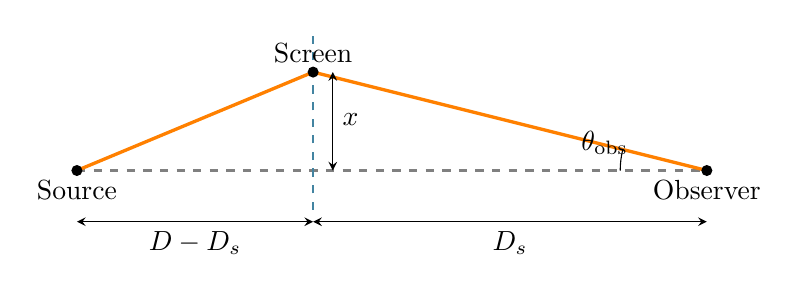
\begin{tikzpicture}[scale=1.0,>=stealth]

    % Coordinates
    \coordinate (S) at (0,0);
    \coordinate (P) at (3,1.25);
    \coordinate (O) at (8,0);

    % Direct path
    \draw[dashed,gray,thick] (S)--(O);

    % Scattered path
    \draw[very thick,orange] (S)--(P)--(O);

    % Screen
    \draw[cyan!60!black,thick,dashed]
        (3,-0.5)--(3,1.8);

    % Points
    \fill (S) circle (2pt);
    \fill (P) circle (2pt);
    \fill (O) circle (2pt);

    % Labels
    \node[below] at (S) {Source};
    \node[below] at (O) {Observer};
    \node[above] at (P) {Screen};

    % Transverse displacement
    \draw[<->]
        (3.25,0)--(3.25,1.25);

    \node[right] at (3.25,0.65) {$x$};

    % Distance labels
    \draw[<->]
        (0,-0.65)--(3,-0.65);

    \node[below]
        at (1.5,-0.65) {$D-D_s$};

    \draw[<->]
        (3,-0.65)--(8,-0.65);

    \node[below]
        at (5.5,-0.65) {$D_s$};

    % Angle at observer
    \draw
        (6.9,0)
        arc[start angle=180,end angle=166,radius=1.1];

    \node at (6.7,0.35) {$\theta_{\rm obs}$};

\end{tikzpicture}
\end{center}

Here $\theta_{\rm obs}$ is the observed
angular offset of the ray from the direct
line of sight.

This is not generally identical to the
deflection angle $\theta_{\rm def}$
produced by the plasma screen.

Using the Pythagorean theorem, the length
of the scattered path is

\begin{equation}
L_{\rm scatt}
=
\sqrt{(D-D_s)^2+x^2}
+
\sqrt{D_s^2+x^2}.
\end{equation}

The direct path has length

\begin{equation}
L_{\rm direct}=D.
\end{equation}

For small scattering angles,

\begin{equation}
x\ll D_s,
\qquad
x\ll D-D_s.
\end{equation}

We can use the Taylor expansion

\begin{equation}
\sqrt{a^2+x^2}
=
a\sqrt{1+\frac{x^2}{a^2}}
\simeq
a+\frac{x^2}{2a}.
\end{equation}

Applying this to both segments,

\begin{align}
L_{\rm scatt}
&\simeq
(D-D_s)
+\frac{x^2}{2(D-D_s)}
+D_s
+\frac{x^2}{2D_s}\\
&=
D+\frac{x^2}{2}
\left(
\frac{1}{D-D_s}
+\frac{1}{D_s}
\right).
\end{align}

The excess path length is

\begin{equation}
\Delta L=L_{\rm scatt}-L_{\rm direct}.
\end{equation}

Therefore,

\begin{equation}
\Delta L=
\frac{x^2}{2}
\left(
\frac{1}{D-D_s}
+\frac{1}{D_s}
\right).
\end{equation}

Combining the fractions,

\begin{equation}
\boxed{
\Delta L=
\frac{x^2D}{2D_s(D-D_s)}.
}
\end{equation}

From the geometry at the observer,

\begin{equation}
\tan\theta_{\rm obs}
=
\frac{x}{D_s}.
\end{equation}

For small angles,

\begin{equation}
\theta_{\rm obs}\simeq\frac{x}{D_s},
\end{equation}

so

\begin{equation}
x\simeq D_s\theta_{\rm obs}.
\end{equation}

Substituting,

\begin{equation}
\boxed{
\Delta L\simeq
\frac{D_sD}{2(D-D_s)}
\theta_{\rm obs}^2.
}
\end{equation}

The additional geometric travel time is

\begin{equation}
\tau_{\rm geom}=\frac{\Delta L}{c}.
\end{equation}

Therefore,

\begin{equation}
\boxed{
\tau_{\rm geom}\simeq
\frac{D_sD}{2c(D-D_s)}
\theta_{\rm obs}^2.
}
\end{equation}

Thus, for a fixed scattering geometry,

\begin{equation}
\boxed{
\tau_{\rm geom}\propto\theta_{\rm obs}^2.
}
\end{equation}

\paragraph{Relating the Observed and Deflection Angles}

To connect this result with our earlier
ray-bending derivation, we must relate
$\theta_{\rm obs}$ to $\theta_{\rm def}$.

The incoming ray travels from the source
to the screen at an angle

\begin{equation}
\theta_{\rm in}\simeq
\frac{x}{D-D_s}
\end{equation}

above the direct line of sight.

After crossing the screen, the ray travels
toward the observer at an angle

\begin{equation}
\theta_{\rm out}\simeq
-\frac{x}{D_s}.
\end{equation}

The net change in propagation direction
at the screen is therefore

\begin{equation}
\theta_{\rm def}
=
\theta_{\rm out}-\theta_{\rm in}.
\end{equation}

Substituting,

\begin{equation}
\theta_{\rm def}
\simeq
-\frac{x}{D_s}
-\frac{x}{D-D_s}.
\end{equation}

Combining the fractions,

\begin{equation}
\theta_{\rm def}
\simeq
-\frac{xD}{D_s(D-D_s)}.
\end{equation}

Since the magnitude of the observed angle is

\begin{equation}
\theta_{\rm obs}\simeq\frac{|x|}{D_s},
\end{equation}

we obtain

\begin{equation}
\boxed{
\theta_{\rm obs}
=
\frac{D-D_s}{D}
|\theta_{\rm def}|.
}
\end{equation}

The observed angle and the physical deflection
angle differ by a geometric factor that is
independent of observing frequency.

We can also express the excess travel time
directly in terms of the deflection angle.

Substituting the above relationship gives

\begin{equation}
\boxed{
\tau_{\rm geom}\simeq
\frac{D_s(D-D_s)}{2cD}
\theta_{\rm def}^2.
}
\end{equation}

This is the usual thin-screen geometric
time-delay relation.

The geometric prefactor depends on the
location of the scattering screen, but not
on the observing frequency.

Consequently,

\begin{equation}
\boxed{
\tau_{\rm geom}\propto\theta_{\rm def}^2.
}
\end{equation}

\subsubsection{The Scattering Index}

We have established two relationships:

\begin{equation}
\theta_{\rm def}\propto\nu^{-2},
\qquad
\tau_{\rm geom}\propto\theta_{\rm def}^2.
\end{equation}

Combining them,

\begin{equation}
\tau_{\rm geom}
\propto
(\nu^{-2})^2.
\end{equation}

Therefore,

\begin{equation}
\boxed{
\tau_{\rm geom}\propto\nu^{-4}.
}
\end{equation}

For a scattering geometry in which the
characteristic angular broadening follows
the same frequency dependence, the
characteristic pulse-broadening timescale
obeys

\begin{equation}
\tau_{\rm scatt}\propto\nu^{-4}.
\end{equation}

Defining the scattering index $\alpha$ by

\begin{equation}
\tau_{\rm scatt}\propto\nu^\alpha,
\end{equation}

we obtain

\begin{equation}
\boxed{\alpha=-4.}
\end{equation}

This result assumes that the characteristic
transverse plasma structure responsible for
deflection is independent of frequency,
and that the scattering geometry remains fixed.

In a turbulent plasma, different observing
frequencies can probe different spatial scales
of the electron-density fluctuations.

For an ideal Kolmogorov electron-density
fluctuation spectrum, the strong-scattering
prediction is instead

\begin{equation}
\boxed{
\alpha=-\frac{22}{5}=-4.4.
}
\end{equation}

Thus, the $\alpha=-4$ result describes
a simple fixed-scale scattering model,
whereas the Kolmogorov prediction accounts
for the scale-dependent structure of
plasma turbulence.
